\subsection*{Lösungen zu Kapitel~\ref{kapitel:Symmediane}: \emph{Symmediane}}

\begin{proof}[Lösung zu Aufgabe~\ref{aufgabe:MEMO2014}]
	Wir beginnen mit einigen Überlegungen, die euch in Fleisch und Blut übergehen sollten, wenn in einer Aufgabe die Gerade durch einen Eckpunkt und den gegenüberliegenden Inkreisberührpunkt vorkommt. Sei $\omega_a$ der Ankreis gegenüber $A$, sei $D_a$ der Berührpunkt von $\omega_a$ mit $\overline{BC}$ und sei $S$ der gegenüberliegende Punkt zu $D_a$ auf $\omega_a$. Dann sind $A$, $D$ und $S$ kollinear, denn die Streckung mit Zentrum $A$, die den Inkreis $\omega$ auf den Ankreis $\omega_a$ abbildet, muss $D$ auf $S$ abbilden. Außerdem erinnern wir uns, dass die Tangentenabschnitte $\overline{CD}$ und $\overline{BD_a}$ am In- und Ankreis gleich lang sind, sodass $M$ auch der Mittelpunkt von $\overline{D_aD}$ ist. Die Gerade $I_aM$ verläuft also sowohl durch den Mittelpunkt $M$ von $\overline{D_aD}$, als auch durch den Mittelpunkt $I_a$ von $\overline{D_aS}$. Folglich muss $I_aM$ parallel zu $AD$ sein. Das sieht schon mal nach einem guten Anfang aus, aber warum $BNCL$ ein Sehnenviereck sein soll, ist daraus noch nicht ersichtlich.
	
	\begin{figure}[ht]
		\centering
		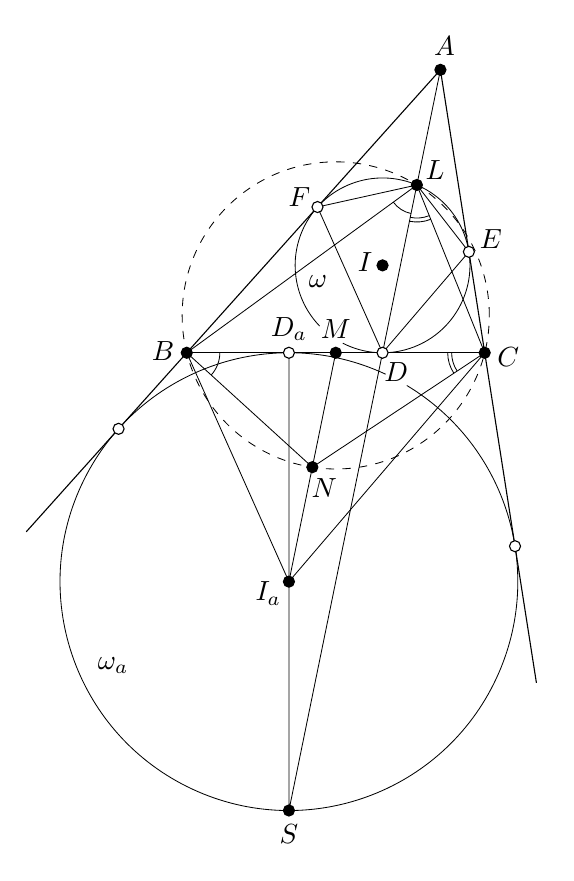
\begin{tikzpicture}[x=0.5cm,y=0.5cm]
			%\clip (-4.66,-6.97) rectangle (5.17,6.77);
			\draw [line width=0.3,shift={(-0.108,2.22)}] (-117:2.22) arc (-117:224:2.22);
			\draw [line width=0.3,shift={(-2.486,-5.813)}]  (65:5.813) arc (65:419:5.813);
			\draw [line width=0.3,dashed] (-1.297,0.949) circle (3.901);
			\coordinate (A) at (1.362,7.187);
			\coordinate (B) at (-5.081,0);
			\coordinate (C) at (2.487,0);
			\coordinate (D) at (-0.108,0);
			\coordinate (E) at (2.085,2.564);
			\coordinate (F) at (-1.76,3.702);
			\coordinate (Da) at (-2.486,0);
			\coordinate (Ea) at (-6.813,-1.932);
			\coordinate (Fa) at (3.257,-4.913);
			\coordinate (I) at (-0.108,2.22);
			\coordinate (Ia) at (-2.486,-5.813);
			\coordinate (L) at (0.764,4.262);
			\coordinate (M) at (-1.297,0);
			\coordinate (N) at (-1.891,-2.906);
			\coordinate (S) at (-2.486,-11.626);
			\draw (B) to (C);
			\draw [shorten >=-5em] (A) to (Ea);
			\draw [shorten >=-5em] (A) to (Fa);
			\draw [line width=0.3] (Da) to (S) to (A);
			\draw [line width=0.3] (Ia) to (B) to (N) to (C) to (Ia) to (M);
			\draw [line width=0.3] (B) to (L) to (E) to (D) to (F) to (L) to (C);
			\draw [line width=0.3,shift={(B)}] (-42.342:0.42cm) arc (-42.342:0:0.42cm);
			\draw [line width=0.3,shift={(L)}] (216.097:0.37cm) arc (216.097:258.439:0.37cm);
			\draw [line width=0.3,shift={(L)}] (258.439:0.42cm) arc (258.439:292.015:0.42cm);
			\draw [line width=0.3,shift={(L)}] (258.439:0.47cm) arc (258.439:292.015:0.47cm);
			\draw [line width=0.3,shift={(C)}] (180:0.42cm) arc (180:213.576:0.42cm);
			\draw [line width=0.3,shift={(C)}] (180:0.47cm) arc (180:213.576:0.47cm);
			\draw [fill=black] (A) circle (2pt) node[shift={(80:2ex)}] {$A$};
			\draw [fill=black] (B) circle (2pt) node[shift={(175:2ex)}] {$B$};
			\draw [fill=black] (C) circle (2pt) node[shift={(-10:2ex)}] {$C$};
			\draw [fill=white] (D) circle (2pt) node[shift={(305:2ex)}] {$D$};
			\draw [fill=white] (E) circle (2pt) node[shift={(30:2.125ex)}] {$E$};
			\draw [fill=white] (F) circle (2pt) node[shift={(150:1.75ex)}] {$F$};
			\draw [fill=black] (I) circle (2pt) node[shift={(170:1.5ex)}] {$I$};
			\draw [fill=black] (Ia) circle (2pt) node[shift={(210:2ex)}] {$I_a$};
			\draw [fill=white] (Da) circle (2pt) node[shift={(90:2ex)}] {$D_a$};
			\draw [fill=white] (Ea) circle (2pt);
			\draw [fill=white] (Fa) circle (2pt);
			\draw [fill=black] (L) circle (2pt) node[shift={(40:2ex)}] {$L$};
			\draw [fill=black] (M) circle (2pt) node[shift={(90:2ex)}] {$M$};
			\draw [fill=black] (N) circle (2pt) node[shift={(300:2ex)}] {$N$};
			\draw [fill=black] (S) circle (2pt) node[shift={(270:2ex)}] {$S$};
			\node at (-1.75,1.8) {$\omega$};
			\node at (-6.95,-7.95) {$\omega_a$};
		\end{tikzpicture}
	\end{figure}
	
	Um die Sehnenviereckseigenschaft nachzuprüfen, müssen wir irgendwie an die Winkel $\winkel BLC$ und $\winkel CNB$ herankommen. Auf den ersten Blick erscheint das hoffnungslos. Aber auf den zweiten Blick eröffnet das Symmedian-Lemma eine Möglichkeit: Wenn $E$ und $F$ die Berührpunkte des Inkreises $\omega$ mit den Seiten $\overline{CA}$ und $\overline{AB}$ sind, dann ist $BL$ der Symmedian durch $L$ im Dreieck $DLF$ und $CL$ ist der Symmedian durch $L$ im Dreieck $DEL$. Andererseits sind $BN$ und $CN$ die Seitenhalbierenden von $\overline{I_aM}$ in den Dreiecken $BI_aM$ und $CMI_a$. Wenn wir zeigen könnten, dass $DLF$ und $BI_aM$ (gegensinnig) ähnlich sind, dann würde also $\winkel BLD=\winkel NBM$ folgen. Analog wäre $\winkel DLC=\winkel MCN$. Mithilfe der Innenwinkelsumme im Dreieck $BNC$ würde also
	\begin{equation*}
		\winkel BLC=\winkel BLD+\winkel DLC=\winkel NBM+\winkel MCN=180^\circ-\winkel CNB
	\end{equation*}
	folgen und wir würden wie gewünscht erhalten, dass $BNCL$ ein Sehnenviereck ist. Die Ähnlichkeit $BI_aM\sim DLF$ ist nun eine einfache Winkeljagd: Weil $BI_a$ die Außenwinkelhalbierende von $\winkel CBA$ ist, gilt $\winkel I_aBM=90^\circ-\beta/2$, wobei wie üblich $\beta\coloneqq \winkel CBA$. Weil die Tangentenabschnitte $\overline{BD}$ und $\overline{BF}$ gleich lang sind, ist das Dreieck $BDF$ gleichschenklig und es gilt $\winkel FDB=90^\circ-\beta/2$. Nach dem Sehnen-Tangentenwinkelsatz ist also auch $\winkel FLD=90^\circ-\beta/2$. Andererseits haben wir schon $I_aM\parallel AD$ bemerkt, sodass $\winkel BMI_a=\winkel CDL$ gilt. Wiederum nach dem Sehnen-Tangentenwinkelsatz ist $\winkel CDL=\winkel DFL$. Also stimmen die Dreiecke $BI_aM$ und $DLF$ in zwei Winkeln überein und sind daher wie gewünscht (gegensinnig) ähnlich.
\end{proof}

\begin{proof}[Lösung zu Aufgabe~\ref{aufgabe:PolenMO2019}]
	Sich berührende Kreise riechen tendenziell nach Inversion, aber bei dieser Aufgabe führt das zu nichts. Der einzige Punkt, an dem wir potentiell invertieren könnten, ohne uns die Aufgabe komplett zu zerschießen, ist $A$. Nach der Inversion berührt $\omega_E'$ die Gerade $\Omega'$, aber auch den Umkreis $\odot AB'E'$, also haben wir es immer noch mit sich berührenden Kreisen zu tun und die Aufgabe ist nicht einfacher geworden (tatsächlich sogar schwerer, weil sich $\omega'$ schwerer beschreiben lässt). Allgemein gilt: Wenn sich in einer Aufgabe Kreise berühren und Inversion zu nichts führt, dann muss stattdessen am Berührpunkt gestreckt werden. Momentan ist noch nicht klar, was das bringt, aber wir behalten es im Hinterkopf.
	
	\begin{figure}[ht]
		\centering
		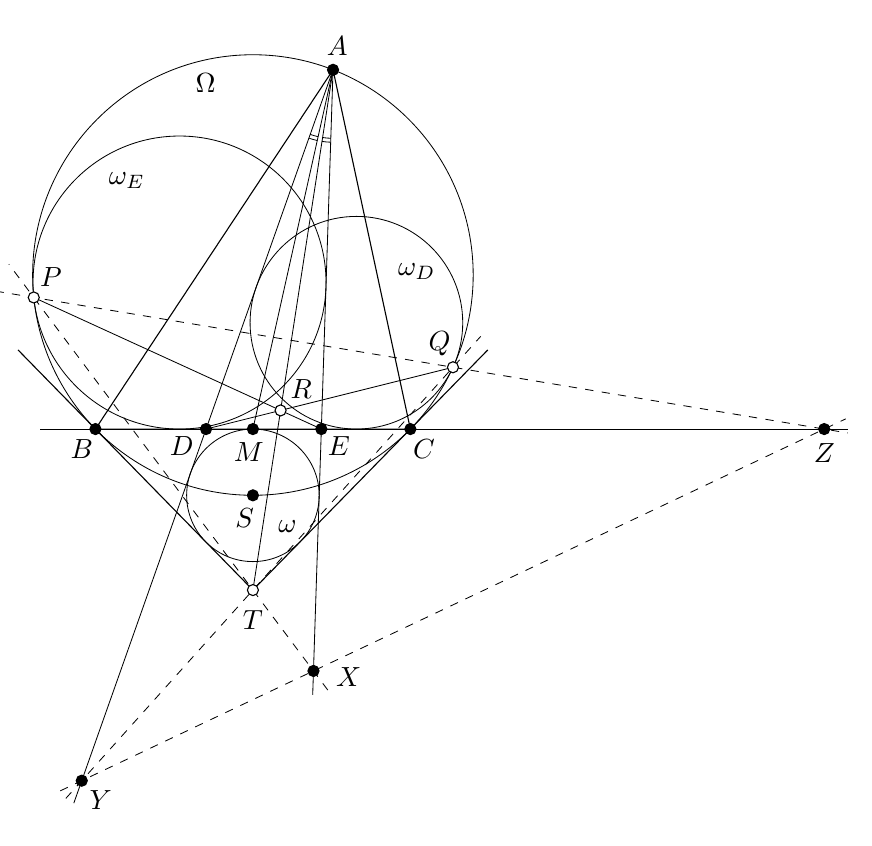
\begin{tikzpicture}[x=0.4cm,y=0.4cm]
			%\clip (-4.66,-6.97) rectangle (5.17,6.77);
			%\draw [line width=0.3,shift={(-0.108,2.22)}] (-117:2.22) arc (-117:224:2.22);
			%\draw [line width=0.3,shift={(-2.486,-5.813)}]  (65:5.813) arc (65:419:5.813);
			\coordinate (A) at (3.544,11.406);
			\coordinate (B) at (-4,0);
			\coordinate (C) at (6,0);
			\coordinate (D) at (-0.488,0);
			\coordinate (E) at (3.173,0);
			\coordinate (M) at (1,0);
			\coordinate (P) at (-5.958,4.178);
			\coordinate (Q) at (7.352,1.962);
			\coordinate (R) at (1.879,0.592);
			\coordinate (S) at (1,-2.104);
			\coordinate (T) at (1,-5.112);
			\coordinate (X) at (2.923,-7.68);
			\coordinate (Y) at (-4.434,-11.164);
			\coordinate (Z) at (19.139,0);
			\draw [line width=0.3] (1,4.891) circle (6.994);
			\draw [line width=0.3] (-1.33,4.652) circle (4.652);
			\draw [line width=0.3] (4.286,3.376) circle (3.376);
			\draw [line width=0.3] (S) circle (2.104);
			\draw (A) to (B) to (C) to cycle;
			\draw [line width=0.3,shorten <=-2ex,shorten >=-1.5em,dashed] (X) to (P);
			\draw [line width=0.3,shorten <=-2ex,shorten >=-1.5em,dashed] (Y) to (Q);
			\draw [line width=0.3,shorten >=-2ex] (A) to (X);
			\draw [line width=0.3,shorten >=-2ex] (A) to (Y);
			\draw [shorten <=-4em] (B) to (T);
			\draw [shorten <=-4em] (C) to (T);
			\draw [line width=0.3,shorten <=-2em,shorten >=-2ex] (B) to (Z);
			\draw [line width=0.3,shorten <=-2em,shorten >=-2ex,dashed] (P) to (Z);
			\draw [line width=0.3,dashed,shorten <=-2ex,shorten >=-2ex] (Y) to (Z);
			\draw [line width=0.3] (A) to (M);
			\draw [line width=0.3] (A) to (T);
			\draw [line width=0.3] (E) to (P);
			\draw [line width=0.3] (D) to (Q);
			\draw [line width=0.3,shift={(A)}] (250.532:0.87cm) arc (250.532:257.425:0.87cm);
			\draw [line width=0.3,shift={(A)}] (250.532:0.92cm) arc (250.532:257.425:0.92cm);
			\draw [line width=0.3,shift={(A)}] (261.243:0.87cm) arc (261.243:268.136:0.87cm);
			\draw [line width=0.3,shift={(A)}] (261.243:0.92cm) arc (261.243:268.136:0.92cm);
			\draw [fill=black] (A) circle (2pt) node[shift={(80:2ex)}] {$A$};
			\draw [fill=black] (B) circle (2pt) node[shift={(235:2ex)}] {$B$};
			\draw [fill=black] (C) circle (2pt) node[shift={(305:2ex)}] {$C$};
			\draw [fill=black] (D) circle (2pt) node[shift={(215:2.5ex)}] {$D$};
			\draw [fill=black] (E) circle (2pt) node[shift={(315:2.07ex)}] {$E$};
			\draw [fill=black] (M) circle (2pt) node[shift={(260:2ex)}] {$M$};
			\draw [fill=white] (P) circle (2pt) node[shift={(50:2.25ex)}] {$P$};
			\draw [fill=white] (Q) circle (2pt) node[shift={(120:2.25ex)}] {$Q$};
			\draw [fill=white] (R) circle (2pt) node[shift={(46:2.5ex)}] {$R$};
			\draw [fill=black] (S) circle (2pt) node[shift={(250:2ex)}] {$S$};
			\draw [fill=white] (T) circle (2pt) node[shift={(270:2.5ex)}] {$T$};
			\draw [fill=black] (X) circle (2pt) node[shift={(350:3ex)}] {$X$};
			\draw [fill=black] (Y) circle (2pt) node[shift={(315:2.25ex)}] {$Y$};
			\draw [fill=black] (Z) circle (2pt) node[shift={(270:2ex)}] {$Z$};
			\node at (2.1,-3.1) {$\omega$};
			\node at (-0.5,11) {$\Omega$};
			\node at (6.2,5) {$\omega_D$};
			\node at (-3,7.9) {$\omega_E$};
		\end{tikzpicture}
	\end{figure}
	
	Als nächstes erinnern wir uns, dass $S$ nach dem Südpolsatz auf der Winkelhalbierenden von $\winkel BAC$ liegt. Die Tangenten von $A$ an $\omega$ liegen symmetrisch bezüglich $AS$, also symmetrisch bezüglich der Winkelhalbierenden von $\winkel BAC$. Statt $\winkel DAM=\winkel RAE$ können wir also auch $\winkel BAM=\winkel RAC$ zeigen. Mit anderen Worten: Wir müssen zeigen, dass $R$ auf dem Symmedian durch $A$ liegt. Nach dem Symmedian-Lemma ist besagter Symmedian genau die Gerade $AT$, wobei $T$ der Schnittpunkt der Tangenten an $\Omega$ in $B$ und $C$ ist. Also zeichnen wir $T$ in unsere Skizze ein -- und siehe da: Es scheint, als ob $\omega$ der Inkreis des Dreiecks $BTC$ ist!
	
	Diese Beobachtung lässt sich durch eine einfache Winkeljagd bestätigen: Nach dem Sehnen-Tangentenwinkelsatz gilt $\winkel TBC=\alpha$, wobei wie üblich $\alpha\coloneqq \winkel BAC$. Nach dem Peripheriewinkelsatz gilt aber auch $\winkel SBC=\winkel SAC=\alpha/2$, weil $S$ auf der Winkelhalbierenden von $\winkel BAC$ liegt. Also liegt $S$ ebenfalls auf der Winkelhalbierenden von $\winkel TBC$ und analog auch auf der Winkelhalbierenden von $\winkel BCT$. Es handelt sich bei $S$ also in der Tat um den Inkreismittelpunkt von $BTC$ und daher bei $\omega$ um den zugehörigen Inkreis.
	
	Nun stecken wir erst einmal fest: Wir müssen zeigen, dass sich die Geraden $AT$, $DQ$ und $EP$ in einem Punkt (nämlich in $R$) schneiden, aber es ist schwer, an diese Geraden heranzukommen. Eine Idee wäre, $\omega$ als Ankreis von $ADE$ zu betrachten. Aus dem Satz von Ceva folgt leicht, dass sich in jedem Dreieck die drei Geraden durch einen Eckpunkt und den gegenüberliegenden Ankreisberührpunkt in einem Punkt schneiden (dem \emph{Nagel-Punkt}). Ihre Spiegelbilder an den Winkelhalbierenden schneiden sich dann ebenfalls in einem Punkt (dem isogonal konjugierten Punkt zum Nagel-Punkt). Mithilfe einer genauen Skizze werdet ihr aber feststellen, dass $DQ$ und $EP$ nicht mit diesen Spiegelbildern übereinstimmen. So kommen wir also nicht weiter.
	
	Wenn ihr feststeckt, dann könnt ihr immer versuchen, mit einem der vielen projektiven Hilfsmittel die Aufgabe umzuformulieren. Hier erinnern wir uns an den Satz von Desargues: Die Geraden $AT$, $DQ$ und $EP$ schneiden sich genau dann in einem Punkt, wenn der Schnittpunkt $X$ von $AE$ und $PT$, der Schnittpunkt $Y$ von $AD$ und $QT$ sowie der Schnittpunkt $Z$ von $BC$ und $PQ$ kollinear sind. Um das zu zeigen, betrachten wir zuerst den Punkt $X$ und erinnern uns, dass wir noch nicht an $P$ gestreckt haben. Das wollten wir tun, weil es eine Streckung an $P$ gibt, die $\omega_E$ auf $\Omega$ abbildet -- also weil $P$ das \emph{äußere Ähnlichkeitszentrum} der Kreise $\omega_E$ und $\Omega$ ist. Wir haben außerdem gesehen, dass $\omega$ der Inkreis von $BTC$ ist, also $T$ der Schnittpunkt der gemeinsamen äußeren Tangenten von $\omega$ und $\Omega$ und somit das äußere Ähnlichkeitszentrum von $\omega$ und $\Omega$. Nach dem Satz von Monge liegen die drei äußeren Ähnlichkeitszentren der Kreise $\omega$, $\omega_E$ und $\Omega$ auf einer Geraden, sodass $PT$ durch den Schnittpunkt der äußeren gemeinsamen Tangenten von $\omega$ und $\omega_E$ verläuft. Eine dieser äußeren gemeinsamen Tangenten ist $AE$. Also muss $X$, der Schnittpunkt von $PT$ und $AE$, genau das äußere Ähnlichkeitszentrum von $\omega$ und $\omega_E$ sein!
	
	Analog ist $Y$ das äußere Ähnlichkeitszentrum von $\omega$ und $\omega_D$. Eine ähnliche Überlegung mit $\omega_D$, $\omega_E$ und $\Omega$ führt schließlich darauf, dass $Z$, der Schnittpunkt von $PQ$ mit $BC$, das äußere Ähnlichkeitszentrum von $\omega_D$ und $\omega_E$ ist. Also sind $X$, $Y$ und $Z$ die äußeren Ähnlichkeitszentren der Kreise $\omega$, $\omega_D$ und $\omega_E$, welche nach dem Satz von Monge kollinear sind. Also sind wir fertig!
\end{proof}